% no answer key
% \documentclass[letterpaper, portrait]{exam}

% answer key
\documentclass[letterpaper, landscape]{exam}
\usepackage{2in1, lscape} 
\printanswers{}

\usepackage{units} 
\usepackage{parskip} 
\usepackage{xfrac} 
\usepackage[fleqn]{amsmath}
\usepackage{cancel}
\usepackage{float}
\usepackage{mdwlist}
\usepackage{booktabs}
\usepackage{cancel}
\usepackage{polynom}
\usepackage{caption}
\usepackage{fullpage}
\usepackage{comment}
\usepackage{enumerate}
\usepackage{graphicx}

\newcommand{\degree}{\ensuremath{^\circ}} 
\everymath{\displaystyle}


\title{Statistics \\ Homework Four}
\date{\today}
\author{}

\begin{document}

  \maketitle

  \section{Homework}
    \begin{itemize*}
      \item read Chapter 4 
      \item exercises: 25--29, 31--32, 34, 36--39, 43--44
    \end{itemize*}

    \ifprintanswers{}
  \else

    If you don't have a calculator with a correlation button or access to a
    computer that can do correlation, feel free to skip 29c and 32b.  
    
    Figuring out the correlation for a large data set is tedious without a
    computer.  The other problems that ask for correlation only have a few
    points, so figuring it out by hand shouldn't be too bad.

  \fi

  \ifprintanswers{}
    \begin{description}
      \item[25]     
        \begin{enumerate}[(a)]
          \item yes
          \item One student got a 10 out of 100 on the test but estimated
            himself as a 4 out of 5 reader.  
        \end{enumerate}
    
      \item[26]
        \begin{figure}[H]
          \centering
          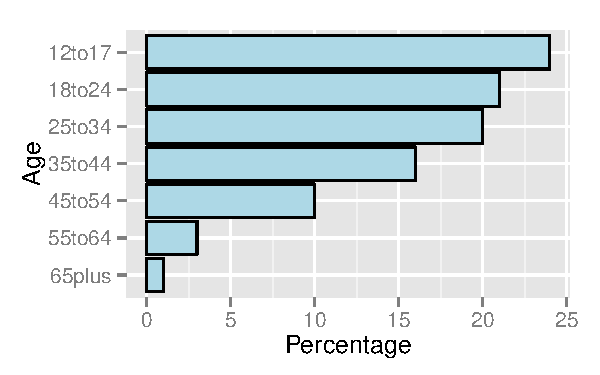
\includegraphics{figures/ex26.pdf}
          \caption{Exercise 26}\label{fig:ex26}
        \end{figure}

        The correlation is 0.5653 so it looks like there is a mild preference
        for tall people to date each other.

      \item[27]
        \begin{figure}[H]
          \centering
          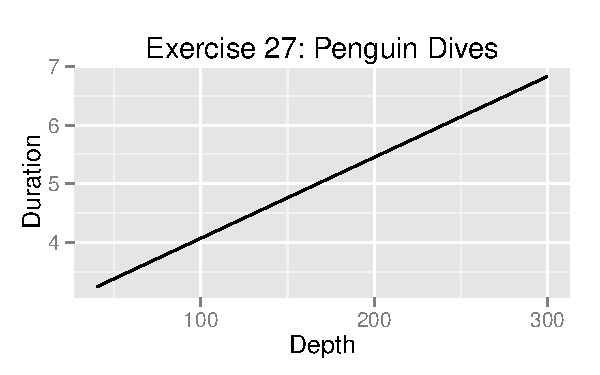
\includegraphics{figures/ex27.pdf}
          \caption{Exercise 27}
        \end{figure}\label{fig:ex27}

        \begin{enumerate}[(a)]
          \item See figure.

          \item
            The correlation is $0.9552$.  There is a strong relationship between the
            coffee price and deforestation.

          \item
            The units of the price don't matter.  Changing the currency would
            just change the labels on the y axis.

        \end{enumerate}

      \item[28]
        \begin{figure}[H]
          \centering
          \includegraphics{figures/ex28.pdf}
          \caption{Exercise 28}
        \end{figure}\label{fig:ex28}

        \begin{enumerate}[(a)]
          \item The correlation is $-0.7485$.  There is a fairly strong negative
            correlation between the number of birds that come back and the
            number of new birds.

            There probably isn't any room for new birds when large numbers of
            returning birds take up all the space.

          \item The sparrowhawk seems to be a long-lived territorial bird.

        \end{enumerate}

      \item[29]
        \begin{figure}[H]
          \centering
          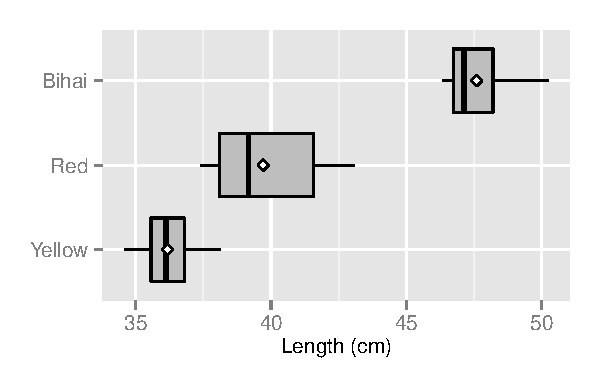
\includegraphics{figures/ex29.pdf}
          \caption{Exercise 29}
        \end{figure}\label{fig:ex29}

        \begin{enumerate}[(a)]
          \item See figure.

          \item
            There is a strong positive correlation with one outlier at (155.2,
            1.94).

          \item
            \begin{tabular}[H]{lr}
              \toprule
              with outlier    & 0.8486 \\
              without outlier & 0.7015 \\
              \bottomrule
            \end{tabular}

            The outlier has large positive z-scores for both neural activity and
            behavior, so it makes a large contribution to the total when
            computing the correlation.

        \end{enumerate}

      \item[31]
        \begin{figure}[H]
          \centering
          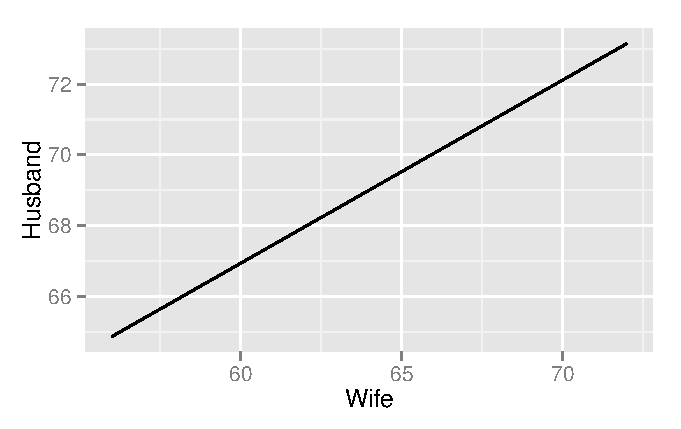
\includegraphics{figures/ex31.pdf}
          \caption{Exercise 31}
        \end{figure}

        There is a strong correlation between time and icicle length.  Not
        surprisingly, if you pour water over an icicle, it gets longer over
        time.

        The more water you pour over the icicle, the more slowly it grows.  This
        is probably because the fast moving water doesn't have as much time to
        freeze.

      \item[32]
        \begin{figure}[H]
          \centering
          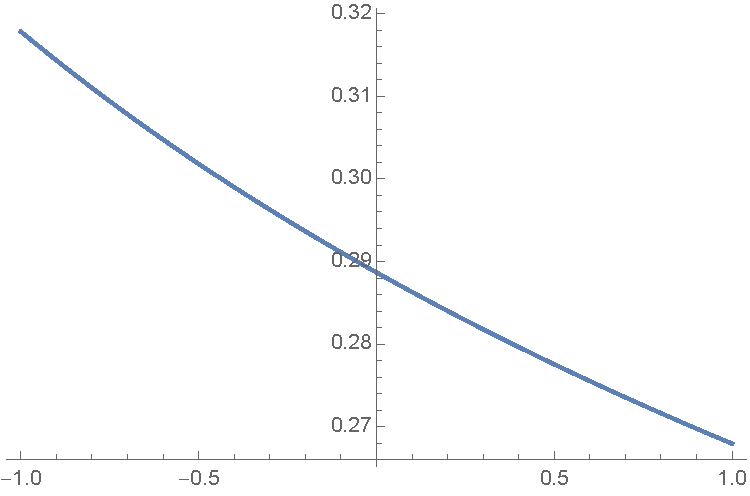
\includegraphics{figures/ex32.pdf}
          \caption{Exercise 32}
        \end{figure}\label{fig:ex32}

        \begin{enumerate}[(a)]
          \item See figure.

          \item The pattern is vaguely linear with a weak positive correlation
            of 0.1349.

          \item When you add the means, you can see that the best choice is
            20,000 plants per acre.

        \end{enumerate}

      \item[34]
        \begin{enumerate}[(a)]
          \item Changing the units would just change the labels on the y-axis.  It
          wouldn't change the correlation.  

          \item Subtracting 6 from all the men's heights doesn't change the
            correlation either.  This is just like changing the scale.

          The correlation just indicates that women tend to date men of similar
          heights.  It doesn't say anything about whether the women (tall or not)
          tend to date men that are taller than they are.

          \item In this case the correlation would be a perfect 1.
        \end{enumerate}

      \item[36] This might happen if the two funds both invest in companies in
        the same industry but one fund includes primarily large companies and
        the other fund includes primarily small companies.  
        
        The large company stocks are fairly stable so they don't tend to go up
        and down much.  The small company stocks tend to move up and down more.
        Both funds move the same direction because both small and large
        companies do well or badly for the same reasons.

        An investor which didn't want to take risks would invest in the fund
        which only moved 10\%.  He wouldn't make too much money but he also
        wouldn't lose too much money.  Another investor who didn't mind more
        risk might invest in the small company stocks.  He would have a chance
        to make more money, but that would come with a chance to lose more as
        well.


        \begin{figure}[H]
          \centering
          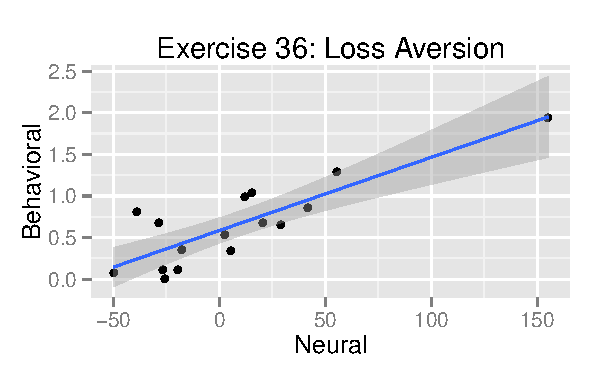
\includegraphics{figures/ex36.pdf}
          \caption{Exercise 36}
        \end{figure}

      \newpage

      \item[37]
        \begin{enumerate}[(a)]
          \item Rachel should invest in small-cap stocks.  When her bonds
            plummet in value, her small-cap stocks are likely to only drop
            slightly.

          \item She should look for a fund with a negative correlation.
        \end{enumerate}

      \item[38]
        The report doesn't say that good researchers make bad teachers.  It just
        says that you can't draw any conclusions about teaching ability from
        research ability and vice versa.  Some excellent researchers are also
        excellent teachers and some excellent researchers are horrible teachers.

      \item[39]
        \begin{enumerate}[(a)]
          \item You can't have a correlation between a categorical variable and
            a quantitative variable.  You need two quantitative variables.

          \item Correlations are always between 1 and -1.

          \item Correlations don't have units.
        \end{enumerate}

      \item[43]
        \begin{figure}[H]
          \centering
          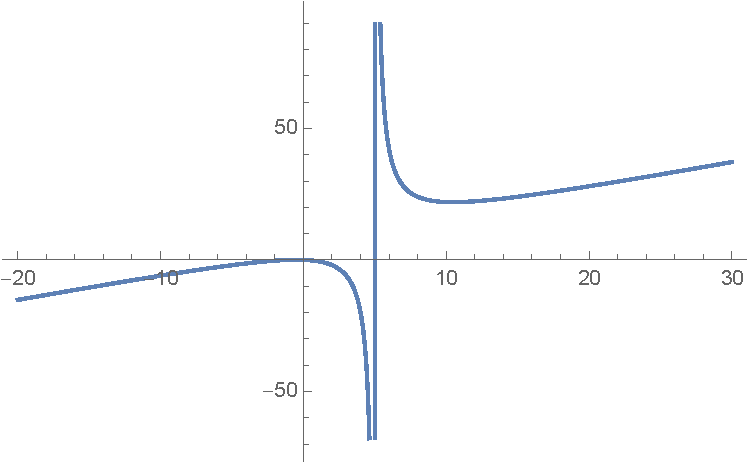
\includegraphics{figures/ex43.pdf}
          \caption{Exercise 43}
        \end{figure}

        It looks like people tend to use about the same gas (not much) in the
        warm months, with or without solar panels.  People with solar panels
        tend to use less gas than people without in the cold months.

        In either case there is a strong positive correlation (0.98) between
        cold months (high degree days) and gas usage.

      \item[44]
        \begin{figure}[H]
          \centering
          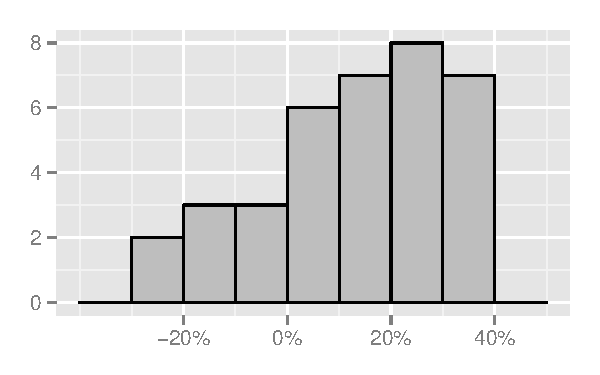
\includegraphics{figures/ex44.pdf}
          \caption{Exercise 44}
        \end{figure}

        There is a fairly strong ($-0.7943$) negative correlation between breeding
        pairs and returning pairs.  The more breeding pairs there are, the fewer
        pairs return each year.

    \end{description}


  \else
    \vspace{10 cm}
    \begin{quote}
      \begin{em}
        The more corrupt a society, the more numerous its laws.
      \end{em}
    \end{quote}
    \hspace{1 cm} --Edward Abbey
  \fi

\end{document}

